%------------------------------------------------------------------------------
\chapter{Sensor Fusion}
\vspace{-1cm} \label{cap3}

%\begin{flushright}
%\begin{minipage}{0.7\linewidth}
%\emph{``Quando uma criatura humana desperta para um grande sonho e
%sobre ele lan�a toda a for�a de sua alma, todo o universo conspira a
%seu favor.''}
%\end{minipage}
%\end{flushright}
%
%\begin{flushright}
%{Goethe}
%\end{flushright}

%\vspace{1cm}

%%Colocar uma descri��o do cap�tulo aqui!
%\section{Introdu��o}\label{sec int_cap_2}


In this chapter, we review sensor fusion techniques, advantages and terminologies. We start with a brief explanation on the motivations of this field of science, grouping them in two main categories: data authenticity and data availability. We continue with a definition of sensor fusion and an exploration on the available fusion method classification models. the four different types: possibilistic, fuzzy reasoning, evidential belief e probabilistic. The latter is further explained, since it is the one used in the simulated examples. Specific techniques to deal with irregular sampling in sensor fusion are also addressed.

\section{Introduction}

The idea that combining information from multiple sensors to improve overall system performances has been in discussion for several decades. In the early days, there were those who argued against the synergism hype that was being spread in military systems, using the multisensor concept \citep{Fowler1979}. In this work, Fowler created what he called his seventh law: 

\begin{quote}
	"Be wary of proposals for synergistic systems. Most of the time when you try to make 2 + 2 = 5, you end up with 3... and sometimes 1.9"
\end{quote}

Although he was right to affirm that the added complexity and high costs are not always worth it - specially back then, when devices were more expensive - many posterior studies advocated that the fusion of sensor data will always be better, in the sense that the probability of correctly classifying a target increases. A direct answer to Fowler's work came in the year after \citep{Nahin1980}, where Nahin and Pokoski used strict concepts and definitions, but also acknowledged the assumptions of discarding network complexity and costs for the sake of their arguments. This topic continued to draw scientific attention throughout the years, like the work of \citep{Rao1998} and \citep{Dasarathy2000}. Rao focused on fusion methods and its comparison to classifiers' performance and establishing conditions that guarantee that the fused system will at least perform as good as the best classifier. Dasarathy's work extended that of Rao's, but was able to show a scenario at which a two-sensor suite outperforms a three sensor suite from a parametric fusion benefits domain perspective. In order to compare performances of fusion levens or algorithm and assess possible benefits of sensor fusion, \citep{Theil2000} discussed three Measures of Performance (MOP), one for each sensor management process, which are Detection, Tracking and Classification.

Despite all philosophical discussions, many real applications have been taking advantage of sensor fusion benefits since the its advent, like remote sensing \citep{Foster1981}, robotics \citep{Richardson1988} and intelligent systems \citep{Luo1989}. Recently, with the modernization and popularization of sensors, its use has grown significantly, with hot topics emerging in the area, such as body sensor networks for health-care applications \citep{Gravina2017}, artificial intelligence \citep{Safari2014, Jordao2018} and smart grids \citep{Liu2012, Kordestani2017}. Recent reviews of the state of the art provide a very broad understanding of the field and its advances \citep{Khaleghi2013, Jing2013}. 

We continue this chapter advocating for the benefits of sensor fusion in Section \ref{sec:motivation}, describing its motivation and advantages In Section \ref{sec:classification}, some of the taxonomy and classifications used in the area are discussed. The type of fusion used in this study is detailed in Section \ref{sec:probabilistic} and we end with the most used techniques in Section \ref{sec:techniques}.


\section{Motivation and Advantages}\label{sec:motivation}

Whether or not all sensor fusion approaches outperform the use of less sensors in every aspect for any given condition, the fact is that many fields of science and engineering have been benefiting from choosing the former.

The reasons why one chooses to fuse information from different sources are various. The works of \citep{Hall1997, Elmenreich2002, Andler2009, Khaleghi2013} provide a detailed study on the motivations and advantages of multi-sensor data fusion techniques. A common benefit from the use of multiple redundant sensors is the increase in accuracy. By averaging all the measurements, the expected error decreases by the rate of $\frac{1}{\sqrt{n}}$, where $n$ is the number of homogeneous sensors, in case of the presence of i.i.d Gaussian noises. Figure \ref{fig:accuracy} illustrates this concept. 

\begin{figure}[!htb]
	\centering
	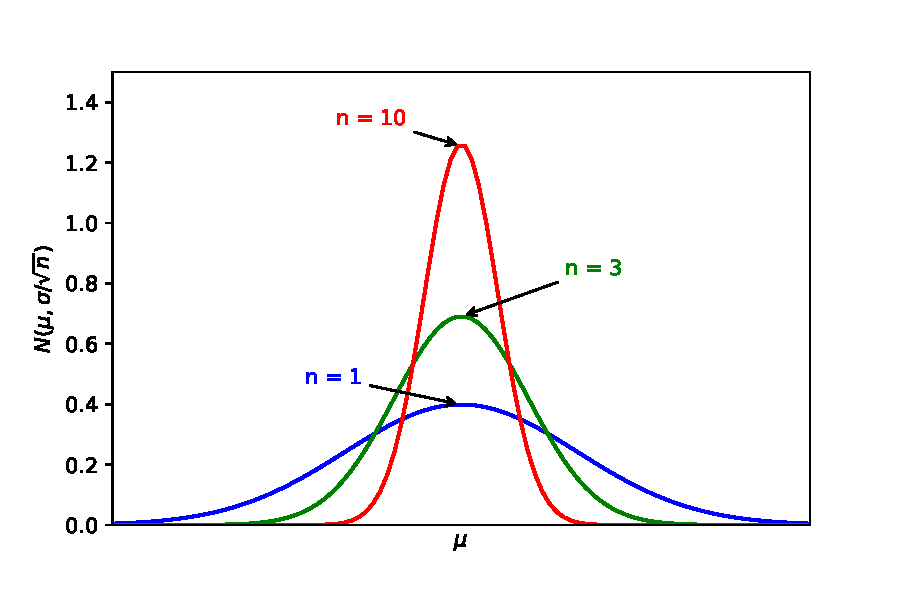
\includegraphics[width=0.75\textwidth]{Imagens/fusion_accuracy.pdf}
	\caption[Probability distribution functions for different amount of fused measurements]{Probability distribution functions for different amount of fused measurements, obtained by 1 (blue), 3 (green) and 10 (red) redundant sensors, considering i.i.d additive Gaussian noise. The higher the value of $n$, the lower is the standard deviation, thus the lower is the expected measurement error.}
	\label{fig:accuracy}
\end{figure}

There are many other reasons to fuse information from multiple sensors, however. Elmenreich gives an interesting example to illustrates some of them. Imagine a car parking assist system with only one distance sensor mounted at its rear, with limited precision and considerable update time (sampling interval). Now picture how would be the system's performance, considering that the sensor may suffer from: deprivation, in the sense that it could be blocked by some physical barrier; coverage, both in spatial and temporal contexts, since it can only sense objects in front of him (spatial) and can only provide information periodically (temporal); precision, with measurement errors being liable to be the cause unexpected bumps; and uncertainty, similarly to what was discussed in Section \ref{sec:uncertain}, when an object, such as a small bicycle, might be missed by the sensor. The system would definitely perform at insufficient levels. All these issues could be solved by adding sensors to the architecture.

Based on the studies from Hall, Elmenreich and Andler, we can group most of the advantages in two categories: Authenticity and Availability improvements. The first group refers to those benefits that improve the quality of the measurement, whereas the second one encompasses those benefits regarding ranges or data dimensions. The addition of sensors can also be of different types (heterogeneous) or of the same type (homogeneous), with redundant measurements. There may be benefits that are exclusive to the addition of different sensors, others exclusive to the addition of redundant sensors and those that can happen both ways. Figure \ref{fig:advantages} presents a schematic with the different advantages expected in sensor fusion.

\begin{figure}[!htb]
	\centering
	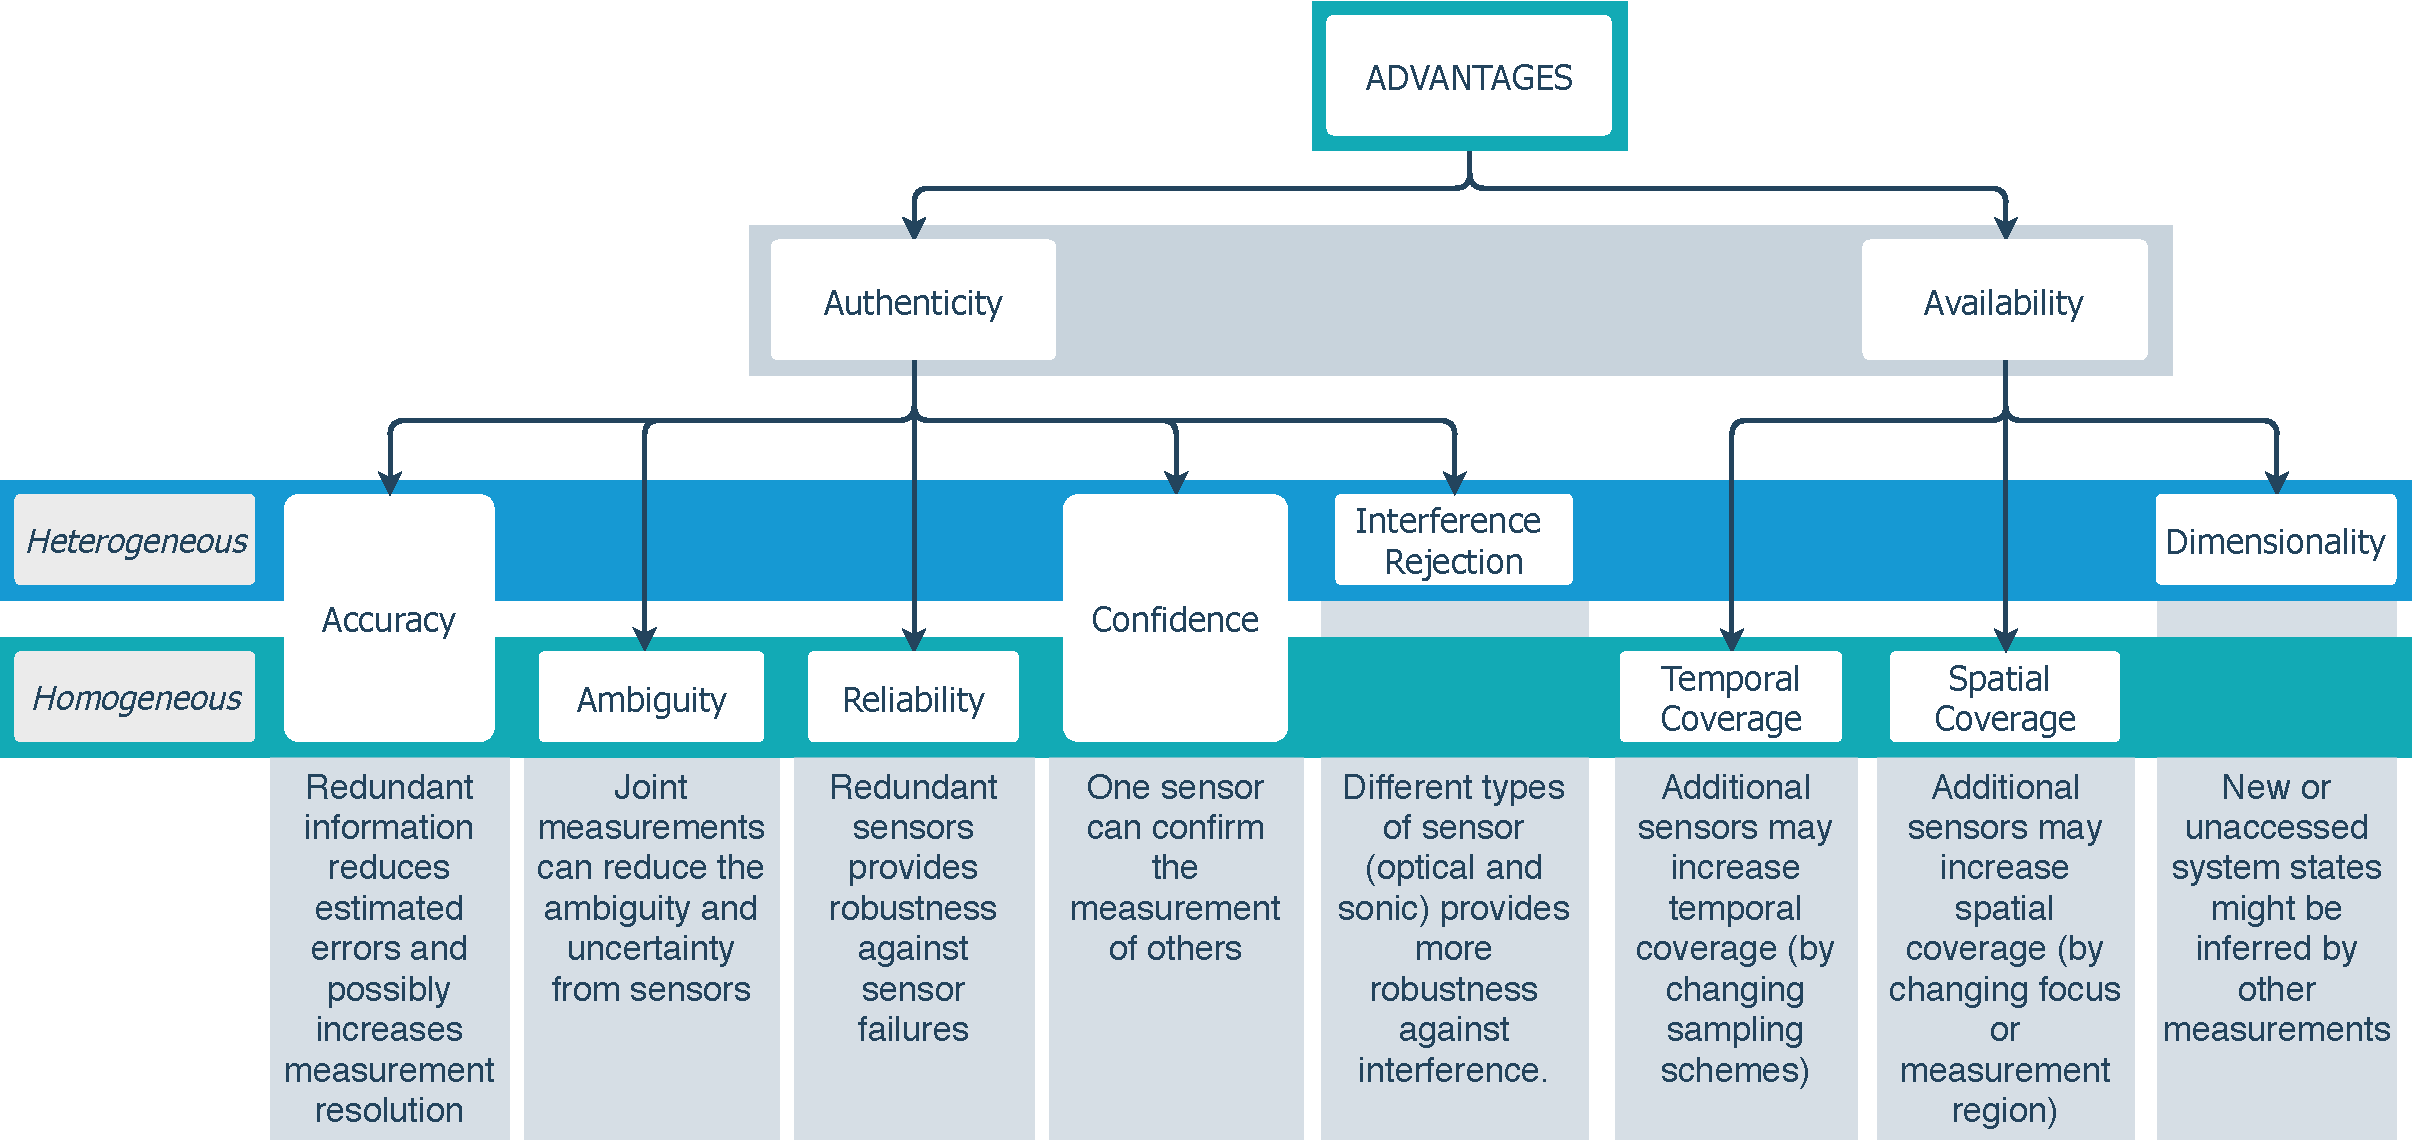
\includegraphics[width=\textwidth]{Imagens/fusion_advantages.pdf}
	\caption[Expected advantages in sensor fusion]{Sensor fusion categorization hierarchy based on expected advantages.}
	\label{fig:advantages}
\end{figure}


\section{Taxonomy and Classification}\label{sec:classification}

Sensor fusion definitions have evolved throughout the years. \citep{Bostrom2007} analyses more than 30 papers on this matter - many of which referenced in this study - to propose a more comprehensible and precise definition to the broad area of information, data and sensor fusion, which we reproduce here:

\begin{quote}
	"Information fusion is the study of efficient methods for automatically or semi-automatically transforming information from different sources and different points in time into a representation that provides effective support for human or automated decision making."
\end{quote}

Researchers in the field made additional efforts to categorize the fusion techniques, using different approaches. One of the earliest attempts comes from \citep{Durrant1988}, where he considered the dynamic use of information in the fusion processes, creating the so called dependence model, which grouped sensor fusion in three categories: competitive, complementary and cooperative. Competitive type occurs when multiple sensors measures the same properties, usually referred to as redundant architecture. Complementary fusion describes the scheme of different types of sensors measuring different information about the same global object or feature, enabling a more complete fused information, like multiple cameras covering a large area. And the last category, cooperative fusion, happens when more complex data are combined to provide information that would not be available (or hard to obtain) otherwise. An example would be multiple measurements processed as softs sensors. A illustrative schematic is presented in Figure~\ref{fig:cat_input}. An abstraction from the human sensory system to Whyte's model is by understanding the way flavors are perceived by our taste (tongue) and smell (nose) sensors in a cooperative fashion. 

\begin{figure}[!htb]
	\centering
	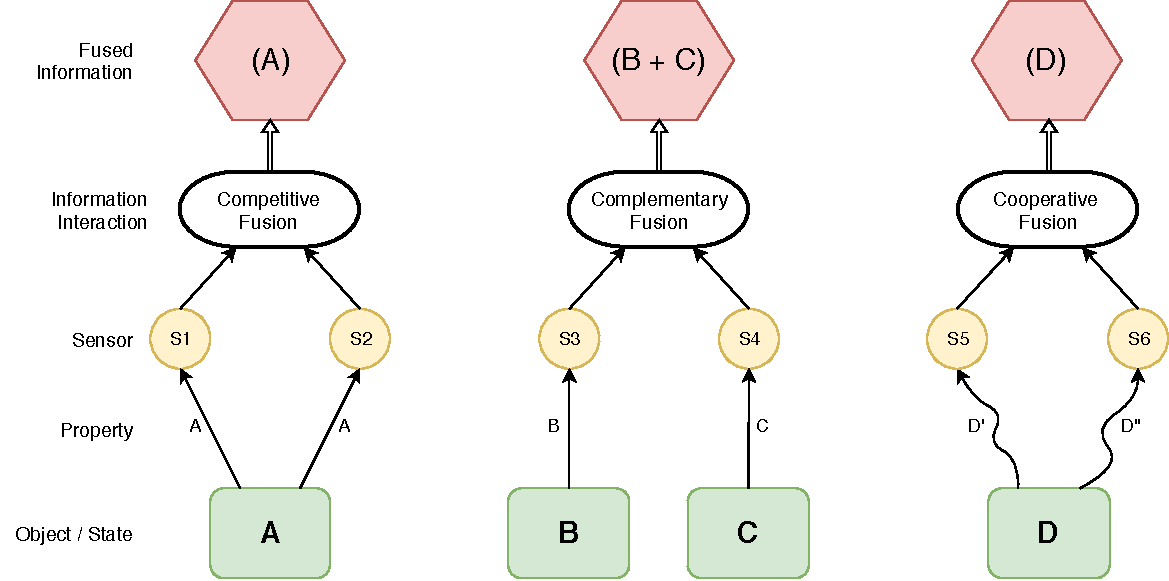
\includegraphics[width=\textwidth]{Imagens/fusion_cat_input.pdf}
	\caption{Classification of data fusion based on sensor interaction.}
	\label{fig:cat_input}
\end{figure}

Another common way to categorize sensor fusion is by the three-level hierarchy based on input / output characteristics, which depends on the processing stage that information is fused. The lower-level is related to raw-data fusion, where signals from sensors are combined. The mid-level is usually related to feature fusion, where information about characteristics of the object are used in the process. The higher level involves decision-fusion, that can be understood as a reasoning process, like the methods of evidential belief or fuzzy logic. \citep{Dasarathy1997} extended this terminology, proposing five fusion modes, according to Figure~\ref{fig:cat_io}. \textit{Data in - data out fusion} (DAI-DAO), the lowest level fusion, processes raw data and outputs raw data, but with some improvements, such as increased accuracy. \textit{Data in - feature out fusion} (DAI-FEO) extracts features from raw data to describe characteristics of the measured environment. \textit{Feature in - feature out} (FEI-FEO) aims at the refinement of the feature entering the process, similarly to what DAI - DAO does to raw data. \textit{Feature in - decison out} (FEI-DEO) usually performs classification based on a set of features received as inputs. \textit{Decision in - decision out} (DEI-DEO) outputs better global decision based on local, restricted decisions. Using our human brain data fusion analogy, many examples can be framed into Dasarathy's terminology. The processing of raw signal from letters symbols into features such as words and texts can be interpreted as DAI-FEO fusion. On the other hand, the process of assimilating features of objects from our eyes and ears, and fuse this features into a decision about what they are, for instance, is an example of FEI-DEO fusion.


\begin{figure}[!htb]
	\centering
	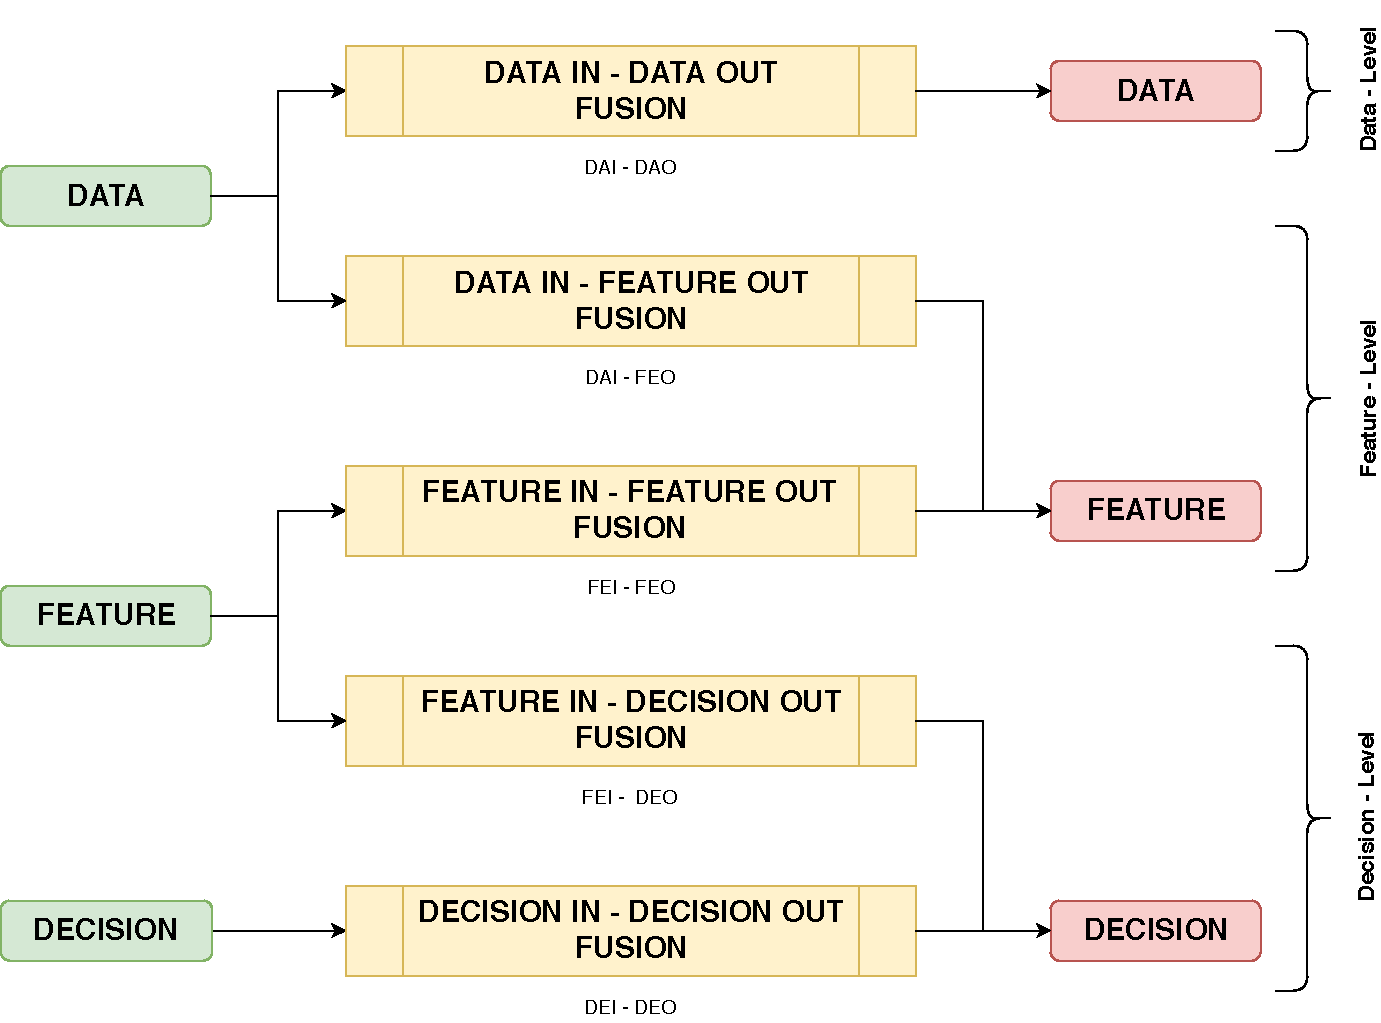
\includegraphics[width=\textwidth]{Imagens/fusion_cat_io.pdf}
	\caption{Input \ Output model and the three fusion levels.}
	\label{fig:cat_io}
\end{figure}

The work of \citep{Castanedo2013} provides a comprehensive review of these and other classification of data fusion techniques. His efforts went beyond as he proposed an interesting new approach, based on the type of architecture, summarized in Figure~\ref{fig:cat_arch}. In his model, fusion techniques that collects all measurements in a central processor lie on the Centralized Architecture category. Assuming perfect data alignment and association, such scheme should be optimal. However it is keen to many sampling irregularities issues and might provoke network congestion. When a network of nodes is used, each with its own processing capability, the architecture becomes decentralized. Such modular strategy ensures scalability, since there are no limits to centralized bottlenecks, and survivability to the loss of a particular sensing node. However it can greatly increase communication costs. The third and last configuration is the distributed architecture, where each data association is performed by local nodes. The separate outputs are then transmitted to a fusion node, that processes these locally obtained estimates to produce a fused global estimate. This scheme will reduce both the communication costs from decentralized architecture and computational costs from the centralized one, while lacking some of their benefits. A fourth architecture could be defined as hierarchical, which combines decentralized and distributed schemes, performing fusion at multiple levels. Getting back to our human sensory capacity, a very complex hierarchical architecture would best describe our fusion scheme in Castanedo's classification.

\begin{figure}[!htb]
	\centering
	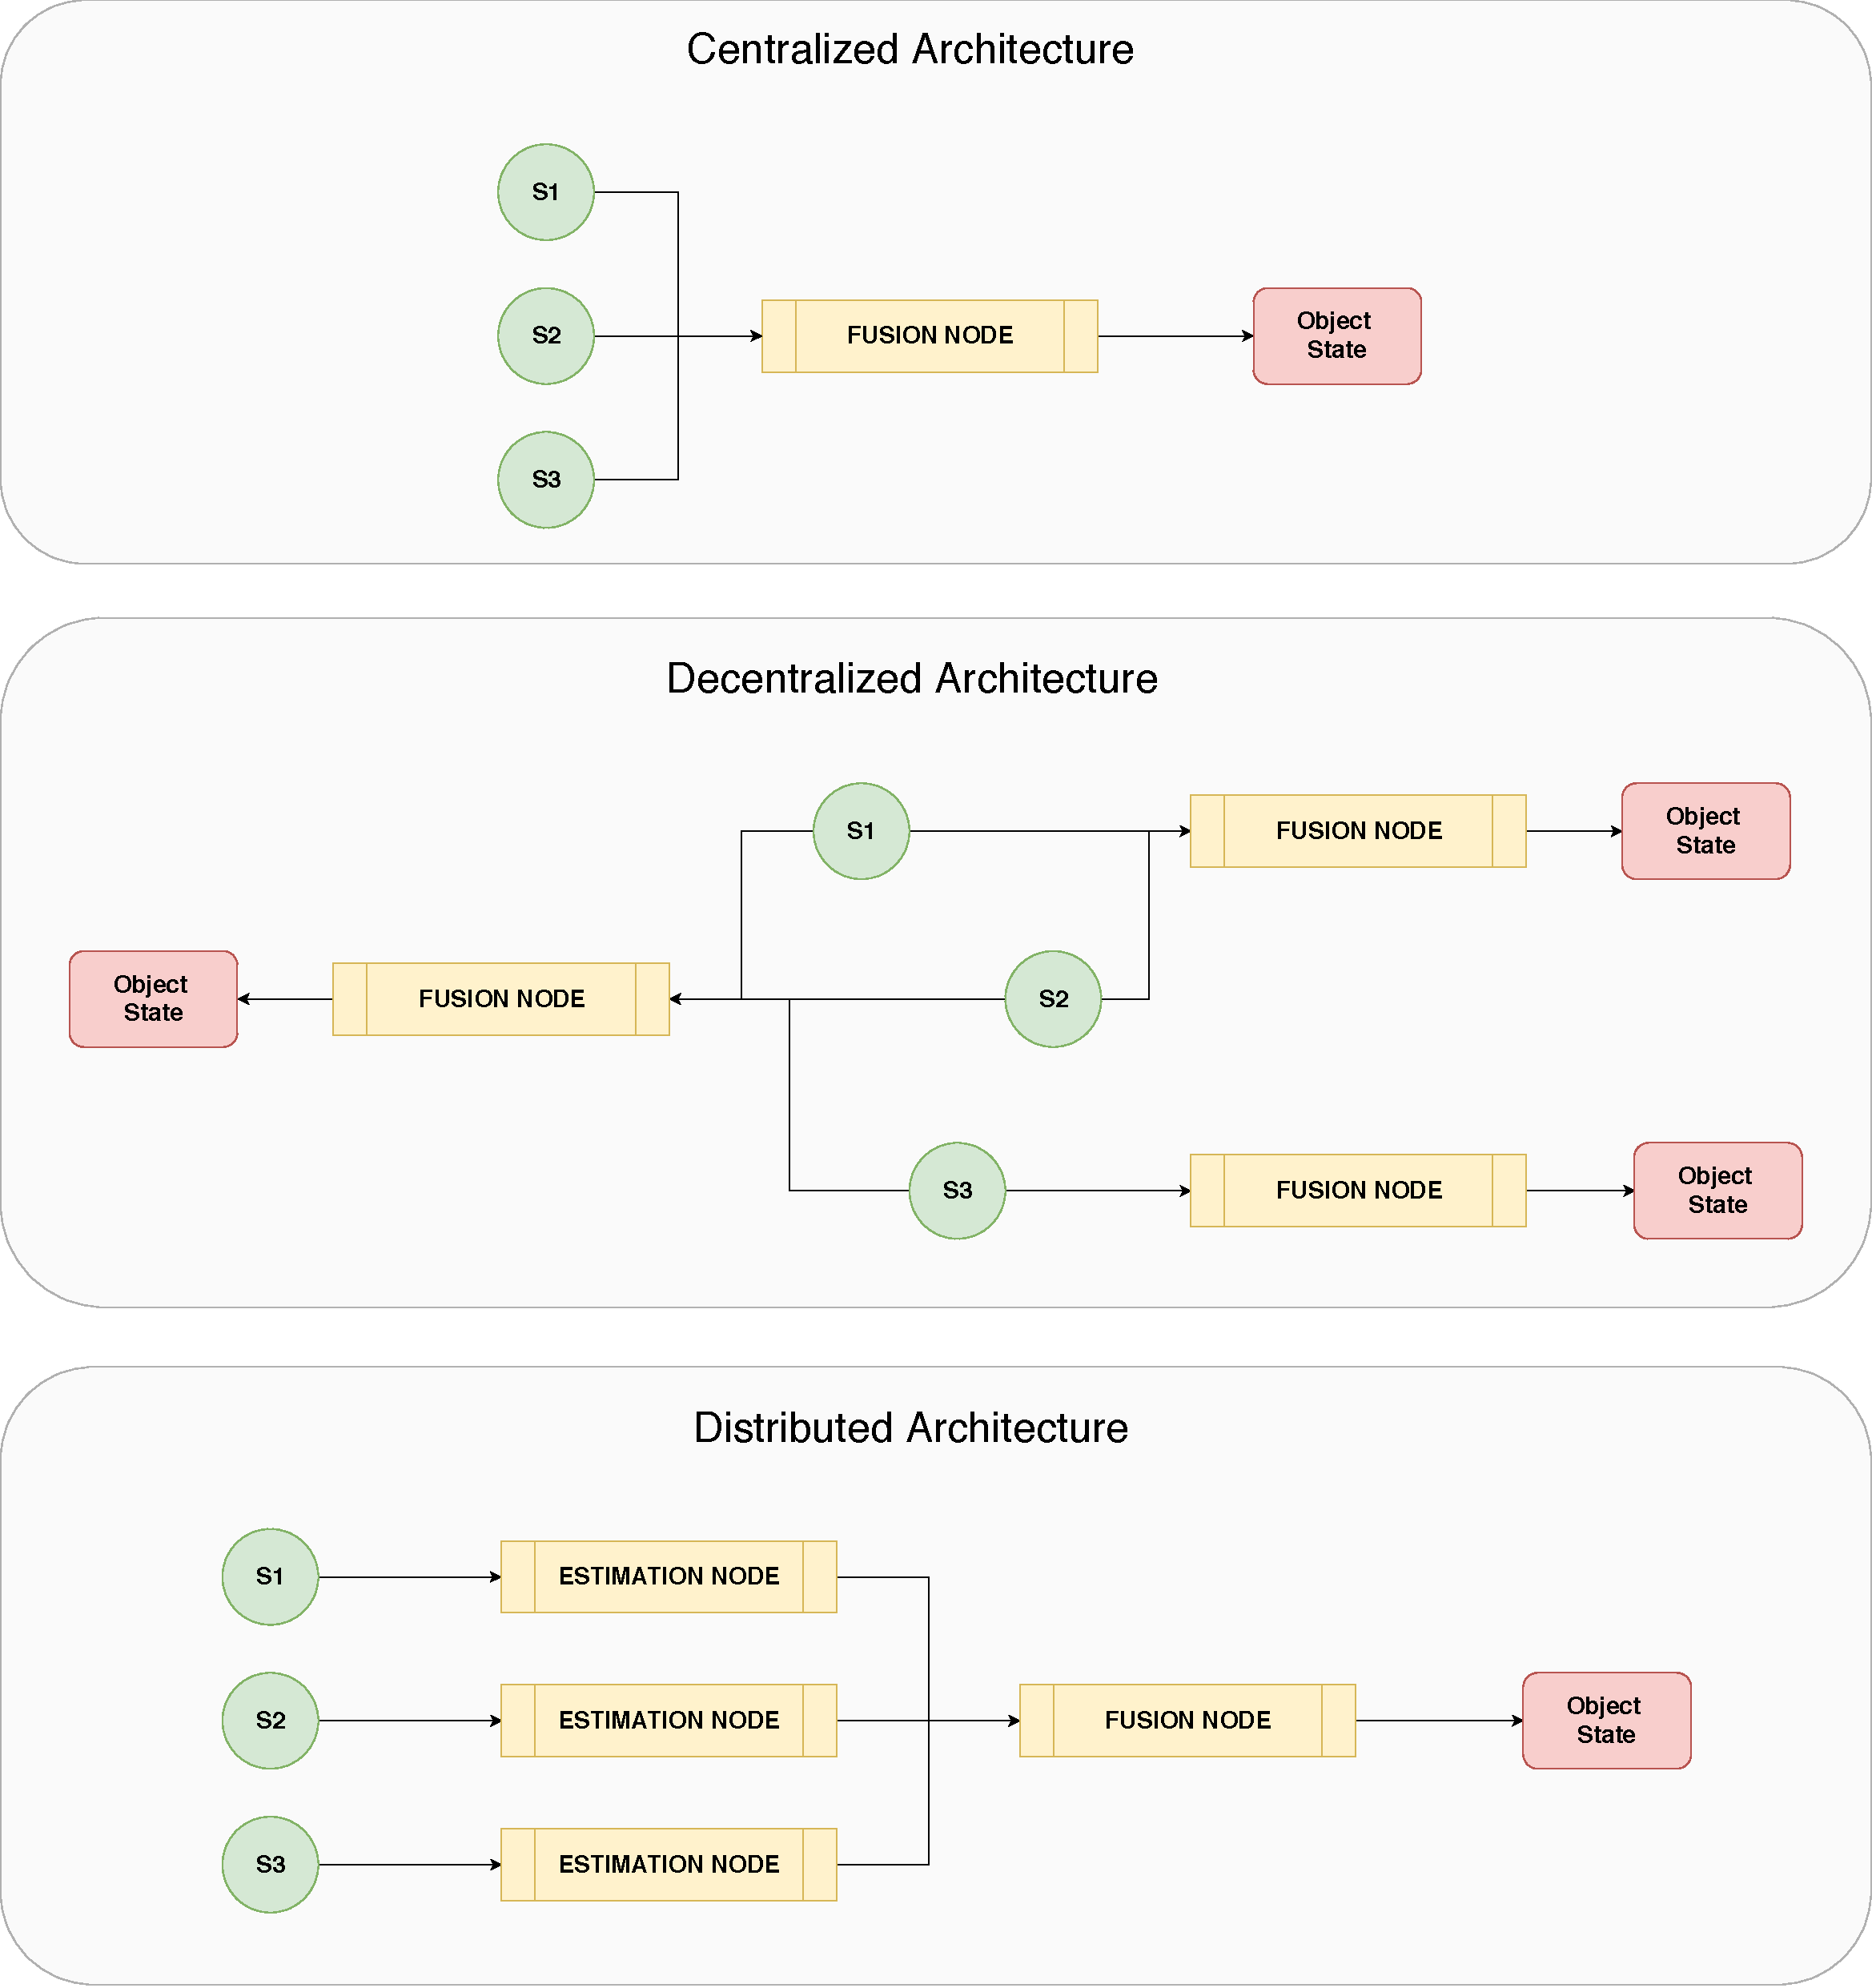
\includegraphics[width=\textwidth]{Imagens/fusion_cat_arch.pdf}
	\caption{Sensor network architectures for data fusion.}
	\label{fig:cat_arch}
\end{figure}

A final note on the taxonomy of data fusion methodologies will be given to the work of \citep{Khaleghi2013}, since it has some connection to sensor fusion in the presence of irregularities, like the ones discussed in Chapter \ref{cap2}. The idea was to study the methods based on data-related challenges they address. An overview of the challenge hierarchy proposed by the authors is presented in Figure~\ref{fig:fusion_challenge}, with four main categories of how challenging input data can be: imperfect, correlated, inconsistent and disparate. The most fundamental problem present in data is imperfection. Indeed, most of the algorithms framed in the other three categories are basically methods that try to neutralize, avoid or minimize their challenges, so that imperfection is the only thing left on data. When correlation is present on data, for instance, the requirements for typical algorithms such as the Kalman Filter, like data independence, are broken, so there are methods to eliminate correlation ora to minimize its effects, given certain assumptions. In case of data inconsistency, due to outliers, one can act on the sensor outputs directly, to validate information or to detect and remove them automatically. If there is out-of-sequence measurements (OOSM) in data, usual frameworks would be to ignore, reprocess or use backward/forward prediction, or apply sate augmentation to incorporate delayed measurements. Conflicted and disparate data are more specific and are beyond the scope of this study.

\begin{figure}[!htb]
	\centering
	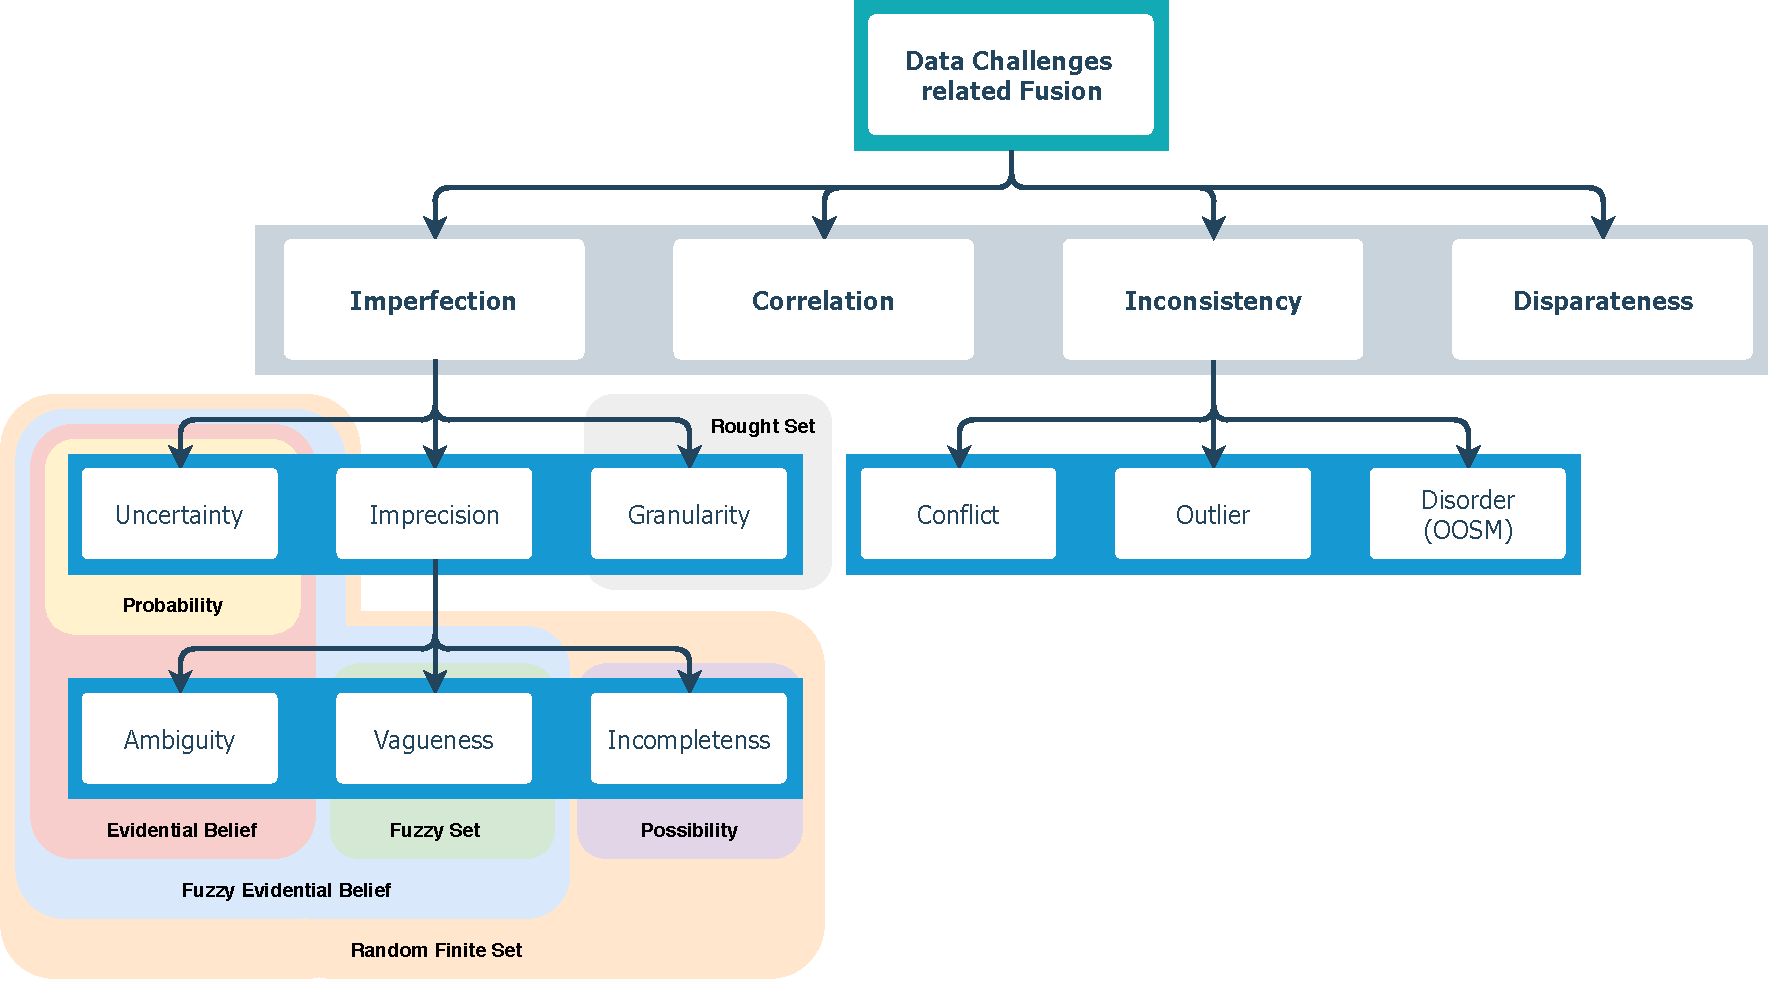
\includegraphics[width=\textwidth]{Imagens/fusion_challenge2.pdf}
	\caption[Data fusion categorization based on data challenges hierarchy]{Categorization based on data challenges hierarchy. For imperfect data, fusion methods and the issues they deal with are also presented.}
	\label{fig:fusion_challenge}
\end{figure}


Being the most fundamental and common challenge present on data, imperfection is also the main focus for research in the area. Based on Khaleghi's classification, imperfection on data can be manifested as uncertainty, imprecision and granularity. We can distinguish uncertainty and imprecision with two information examples: \textit{I believe Mary is one point eight meter tall}; \textit{I am sure that Mary is tall}. In the first sentence, the information is precise, but uncertain. In the second, the information about Mary's height is certain, but imprecise, with some vagueness (fuzziness) attached to it. Usually the amount of precision in data is inversely proportional to the level of certainty. The source of imprecision can also be ambiguity, as in the phrase: \textit{Mary delivered her baby at 5 yesterday}. We don't know if it was 5 p.m. or 5 a.m., though the information was certain. The last type of imprecision would be for incomplete data, when we have missing information. The sentence "\textit{Mary's height is above one point five meter}", is incomplete, for an example, meaning that only one bound was given. Any height above one hundred and fifty centimeters is possible and any height less than or equal to it is impossible, defining the so called possibility measures. Finally, granularity is an imprecision related to the internal structure of data, referring to the ability to distinguish among states. Different attributes on the data or a different set of possible states will generate different levels of imprecise information.

Given the amount of potential problems in data and their particularities, it is only natural that no data fusion approach alone could tackle all of them. Researchers have proposed various approaches that focus on one or a few of the issues and Khaleghi's paper explores methods for all the challenges in his categorization model. In this study we will limit ourselves to imperfect data. Figure~\ref{fig:fusion_challenge} presents an overview of methods that can deal with the sources of imperfection. In most cases, the mathematical background of each method relies on the representation of imperfect data. Uncertainty can be easily modeled by probability distribution functions, thus probabilistic methods are the most adequate to handle it. The most classical approach to fuse data based on uncertain measurements is with Bayes theorem. Considering a sampled-data system with sampling time interval $T$, Bayesian filtering will estimate the states $x_k$ of a system at time instant $kT$ based on the conditional PDF of the state given the set of measurements $Y^k = \{y_1,...,y_k\}$ and its prior distribution and the likelihood function, as following:

\begin{equation}\label{eq:bayes}
\rho(x_k|Y^k) = \frac{\rho(y_k|x_k) \rho(x_k|Y^{k-1})}{\rho(Y^k|Y^{k-1})}
\end{equation}

\noindent
where $\rho(y_k|x_k)$ is the likelihood function, based on the measurement model, $\rho(x_k|Y^{k-1})$ is the prior distribution, given by the system's transition model and the denominator is a normalizing term. For certain conditions, that is linearity and Gaussianity, the Bayes estimator known as Kalman Filter (KF) provides optimal solution and, due to its simplicity it is one of the most popular state estimation method used to fuse data. As such, it is the chosen method for the next sections of this study and will be further discussed later on.



\citep{Florea2007}
\citep{Smets1997}



\begin{table}[!htb]
	% increase table row spacing, adjust to taste
	\renewcommand{\arraystretch}{1.3}
	% if using array.sty, it might be a good idea to tweak the value of
	% \extrarowheight as needed to properly center the text within the cells
	\caption[Data fusion methods for imperfect data]{Data fusion methods for imperfect data. Adapted from \citep{Khaleghi2013}, Table 1, page 35.}
	\label{tabela_transacoes}
	\centering
	% Some packages, such as MDW tools, offer better commands for making tables
	% than the plain LaTeX2e tabular which is used here.
	\begin{flushleft}
	
	{
		\footnotesize
		\begin{tabularx}{\linewidth}{ 	>{\hsize=0.75\hsize}X
										>{\hsize=1.25\hsize}X
										>{\hsize=1.1\hsize}X
										>{\hsize=0.9\hsize}X}
			\hline
			\textbf{Algorithm} 			& \textbf{Approach}    			&  \textbf{Advantages} 		& \textbf{Limitations}\\ 
			\hline
			Probabilistic & Bayesian framework to fuse uncertain data represented by probability distribution functions & Well-established and optimal for certain conditions & Might be unsuited for other data imperfections \\ \\			
			Evidential Belief & Data fusion based on probability mass function, using Dempster-Shafer theory and combination rules & Enables fusion of both uncertain and ambiguous information & Incapable of dealing with other aspects of imperfection \\ \\ 
			Fuzzy Reasoning & Vague data represented by fuzzy set theory and fusion based on fuzzy rules & Intuitive and interpretable approach for vague data, such as human generated & Only applicable to vague data \\ \\
			Possibilistic & Data fusion based on fuzzy theory, with data representation similar to probabilistic and evidential belief & Indicated for poorly informed environment with incomplete data & Not very common and well-established \\ \\
			Rough Set & Imprecise data is approximated based on granularity and manipulated via classical set theory & Dispenses preliminary or additional information & Data granularity must be adequate \\ \\
			Random Set & Extension of Bayesian filter, representing the state space as a random set to capture many aspects of imperfection & Can potentially provide a unified framework for fusion of imperfect data & Not very appreciated by the fusion community \\ \\ 
			Hybridization & Combination of different fusion methods and data representation & More comprehensive treatment of data imperfection and benefits from complementary fusion & Computational expensive and very problem specific \\
		\end{tabularx}
	}
	\end{flushleft}
\end{table}



\section{Probabilistic Sensor Fusion}\label{sec:probabilistic}

Entrar em maiores detalhes do probabilistic, explicando KF e o PF (caso seja utilizado no trabalho).

\subsection{Probabilistic Sensor Fusion Techniques}\label{sec:techniques}

Para fus�o de informa��es m�ltiplas de observa��es, explicar os quatro grandes grupos: parallel filter (multi-output system, multi-output KF), sequential filter (kfusing first output as the prediction for the secod output), outputs fusion (outputs are fused using the noise covariance) e track-to-track fusion (single-output KFs fused considering correlation). \citep{Willner1976,Fatehi2017}

Tentar agrupar os principais m�todos de filtragem, por tipo de irregularidade (possivelmente uma grande tabela)


\clearpage